\documentclass{beamer}

\usepackage[utf8]{inputenc}
\usepackage{csquotes}
\usepackage{latexsym,amsmath,xcolor,multicol,booktabs,calligra, animate, subfig}
\usepackage{graphicx,pstricks,listings,stackengine, bbm}
\usepackage{tikz}
\usetikzlibrary{fit,tikzmark}   
\usepackage{booktabs,cellspace}
\usepackage{color, colortbl}
\usepackage{hyperref}
\usepackage{color}
%Information to be included in the title page:
\title{Air Pollution from Electricity Production}
\author{Lauren Beatty\\ \href{mailto:lbeatty@edf.org}{lbeatty@edf.org}}
\institute{Environmental Defense Fund}
\date{\today}


%% Tikz
\usepackage{tikz}
\usetikzlibrary{shapes.geometric, arrows}

\tikzstyle{start} = [rectangle, rounded corners, 
minimum width=3cm, 
minimum height=1cm,
text centered, 
draw=black, 
fill=orange!30]

\tikzstyle{process} = [rectangle, 
minimum width=3cm, 
minimum height=1cm, 
text centered, 
text width=3cm, 
draw=black, 
fill=blue!30]

\tikzstyle{stop} = [rectangle, rounded corners, 
minimum width=3cm, 
minimum height=1cm,
text centered, 
draw=black, 
fill=green!30]

\tikzstyle{arrow} = [thick,->,>=stealth]


\logo{\includegraphics[height=.5cm]{EDF_color_webRGB_2022 (2).png}\hspace*{.03\paperwidth}\vspace{.01\paperwidth}}


%Color Pallete
\definecolor{EDFblue}{RGB}{0.0, 51, 204}
\definecolor{EDFgreen}{RGB}{0, 153, 51} 
\definecolor{EDFlightgreen}{RGB}{161, 226, 20}
\definecolor{EDFcyan}{RGB}{51,204,255}
\setbeamercolor{structure}{fg=EDFblue} 
\setbeamercolor{button}{bg=EDFblue,fg=white}
\setbeamertemplate{navigation symbols}{}
\newcommand{\nologo}{\setbeamertemplate{logo}{}} % command to set the logo to nothing


\hypersetup{colorlinks,linkcolor=EDFblue,urlcolor=EDFblue}


\begin{document}

\frame{\titlepage}

\begin{frame}
\frametitle{Introduction}
Two Different Questions / Approaches:
\begin{enumerate}
    \item Downscaling
    \begin{itemize}
        \item \textbf{Question}: How might a particular plan for decarbonization affect air pollution.
        \item \textbf{Method}: Sequentially run a least-cost planning model, then take the outputs of that model and predict pollution.
    \end{itemize}
    \item Endogenous
    \begin{itemize}
        \item \textbf{Question}: What decarbonization plan most dramatically decreases air pollution equitably?
        \item \textbf{Method}: Alter the planning model to minimize pollution subject to a cost constraint.
    \end{itemize}
\end{enumerate}
\vspace{1cm}

\end{frame}


\begin{frame}{Background on Least-Cost Electricity Planning Models}
\begin{center}
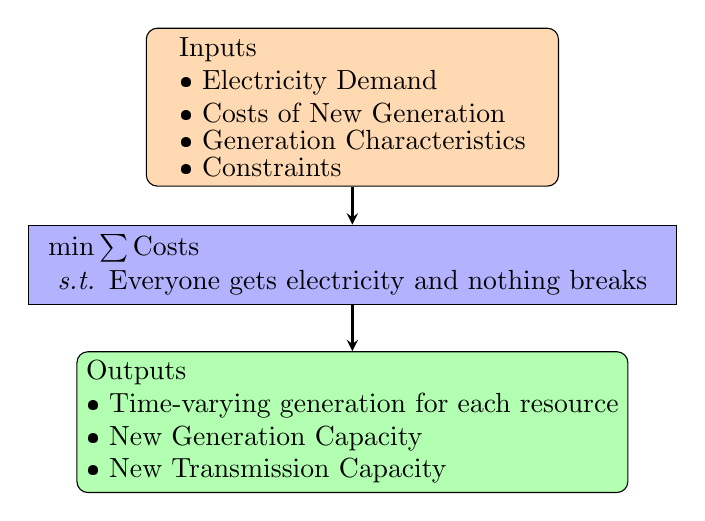
\begin{tikzpicture}[node distance=2cm]
\node (start) [start, text width=5cm] {\shortstack[l]{Inputs\\• Electricity Demand \\ • Costs of New Generation \\ • Generation Characteristics\\
• Constraints}};

\node(obj)[process, below of=start, text width=8cm]{\shortstack[l]{$\min \sum \text{Costs}$ \\ \textit{ 
   s.t.   }\text{Everyone gets electricity and nothing breaks }}};

\node (result) [stop, below of=obj] {\shortstack[l]{Outputs\\• Time-varying generation for each resource \\ • New Generation Capacity \\ • New Transmission Capacity}};

\draw [arrow] (start) -- (obj);
\draw [arrow] (obj) -- (result);

\end{tikzpicture}
\end{center}
\end{frame}

\begin{frame}{Background on Least-Cost Electricity Planning Models: Pros and Cons}
    \begin{itemize}
        \item Powerful for out-of-sample questions

        \item Persuasive in policy arguments.

        \item No or very little backwards validation -- We have no evidence that these models make good predictions about what will happen.

        \item Rely on strong assumptions about future costs and demand, as well as the strong assumption that these are known ex-ante.
    \end{itemize}
\end{frame}

\begin{frame}{Air Pollution Modelling}
\textbf{Translate emissions at points to concentrations over space.} 

\vspace{.3cm}

Multiple models of varying complexity. The main models used in policy work are:
\begin{itemize}
    \item APEEP
    \item INMAP
    \item EASIUR
\end{itemize}

\vspace{.3cm}

These are all \textbf{average-annual models}, with reduced-form representations of more complex chemical transport models. Each answers the question: \textit{How much does pollution affect average annual exposure?} Therefore, they are suitable for thinking about policies affecting aggregate emissions, but not suitable for thinking about things like hourly NAAQs.
\end{frame}

\begin{frame}{Downscaling}
\begin{enumerate}
    \item Run least-cost planning model
    \item Model outputs annual generation for each ``resource," such as Combined Cycle Plants in New England ISO North.
    \begin{itemize}
        \item How much resources are aggregated is a user choice which needs to balance computational feasibility and model accuracy.
    \end{itemize}
    \item Translate model outputs into point source locations and aggregate emissions of important pollutants (in InMAP -- PM2.5, NOx, SOx, VOCs, NH3).
        \begin{itemize}
            \item Involves lots of assumptions about how to allocate generation to existing plants, and the location of new plants.
        \end{itemize}
    \item Run those aggregate emissions through an air pollution model of your choice.
    \item Translate concentrations into health impacts.
\end{enumerate}
\end{frame}

\begin{frame}{MIP Results}
    \begin{columns} % Create two columns
        \column{0.5\textwidth} % First column: 50% of slide width
        \centering
        \includegraphics[width=\linewidth]{Figures/Output/full-base-200/GenX/ISRM_2027_TotalPM25_concentrationmap.jpg}
        \captionof{figure}{PM2.5 Concentrations in 2027 in the base-200 scenario}

        \column{0.5\textwidth} % Second column: 50% of slide width
        \centering
        \includegraphics[width=\linewidth]{Figures/Output/full-base-200/GenX/ISRM_2050_TotalPM25_concentrationmap.jpg}
        \captionof{figure}{PM2.5 Concentrations in 2050 in the base-200 scenario}
    \end{columns}
\end{frame}

\begin{frame}{MIP Results}
    \includegraphics[width=\textwidth]{Figures/Output/Compare_scenarios_current-base_GenX.jpg}
\end{frame}


{\nologo
\begin{frame}{Endogenous Exposure}
    \begin{center}
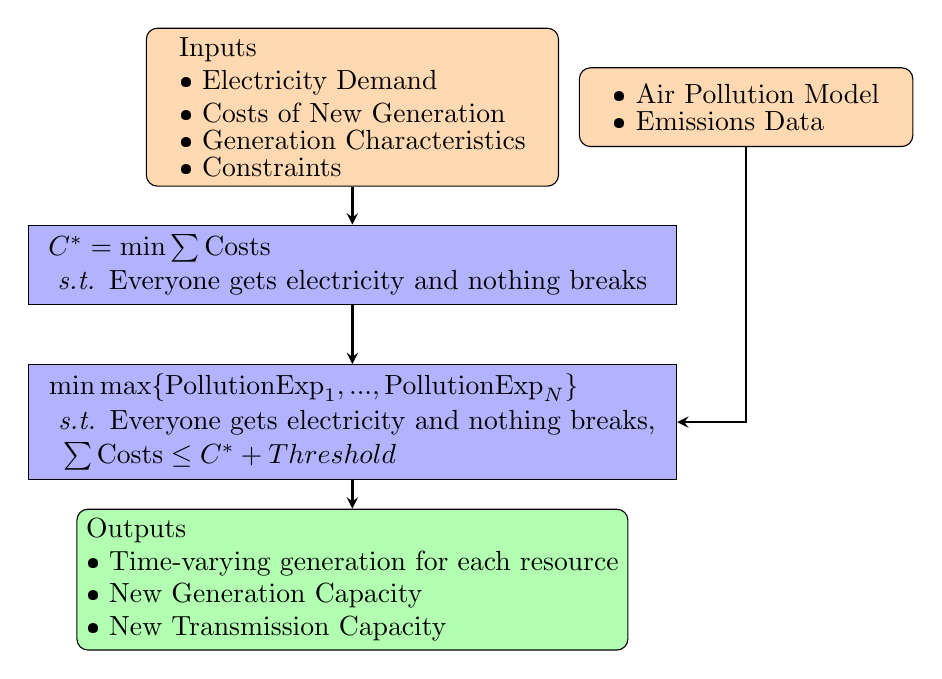
\begin{tikzpicture}[node distance=2cm]

\node (start) [start, text width=5cm] {\shortstack[l]{Inputs\\• Electricity Demand \\ • Costs of New Generation \\ • Generation Characteristics\\
• Constraints}};

\node (air) [start, text width=4cm, right of= start, xshift=3cm] {\shortstack[l]{• Air Pollution Model\\
• Emissions Data}};

\node(obj)[process, below of=start, text width=8cm, xshift=0cm]{\shortstack[l]{$C^* = \min \sum \text{Costs}$ \\ \textit{ 
   s.t.   }\text{Everyone gets electricity and nothing breaks }}};

\node(obj2)[process, below of=obj, text width=8cm, xshift=0cm]{\shortstack[l]{$\min \max\{\text{PollutionExp}_1,...,\text{PollutionExp}_N\}$ \\ \textit{ 
   s.t.   }\text{Everyone gets electricity and nothing breaks,} \\
    $\text{      }\sum \text{Costs} \leq C^*+Threshold$ }};

\node (result) [stop, below of=obj2] {\shortstack[l]{Outputs\\• Time-varying generation for each resource \\ • New Generation Capacity \\ • New Transmission Capacity}};

\draw [arrow] (start) -- (obj);
\draw [arrow] (air) |- (obj2);
\draw [arrow] (obj) -- (obj2);
\draw [arrow] (obj2) -- (result);


\end{tikzpicture}
\end{center}
\end{frame}}


\begin{frame}{Our Approach}
    \begin{enumerate}
        \item Use EPA emissions data to calculate emissions rates (Pounds per MWh)
        \item Use InMap Source-Receptor Matrix to calculate how one MWh of generation for each resource affects population-weighted average exposure for different groups.
        \item Use Switch to calculate least-cost planning costs.
        \item Modify and run Switch to minimize air pollution exposure subject to a cost constraint.
    \end{enumerate}

\paragraph{Benefits}
\begin{itemize}
    \item Avoids the use of equity weights while still centering distributional concerns.
    \item Still finds low-cost solutions.
    \item Generalizable framework
\end{itemize}
\end{frame}

\begin{frame}{A Point About Calculus}
    \includegraphics[width=0.48\textwidth]{Figures/Slide Pictures/Transmission1.png} \includegraphics[width=0.48\textwidth]{Figures/Slide Pictures/Transmission2.png}

    The effect of deviations from the least-cost optimum will depend on the shape of the objective function.  This is an \textit{empirical} question!\\
    \vspace{.5cm}
    $\Rightarrow$ Perhaps you can get large improvements in health at only modest increases in cost.
\end{frame}

\begin{frame}{Flavor of Results}
    \centering
    \includegraphics[width=0.8\textwidth]{Figures/EndogenousResults/current_policies_short_simplified/exposure_cost_PPF.png}
\end{frame}

\begin{frame}{Thanks!}
\label{Thanks}


    Please feel free to contact me at:
    \href{mailto:lbeatty@edf.org}{lbeatty@edf.org}\\
    \vspace{1cm}
\end{frame}
\end{document}